\chapter{Prozess}
\label{ch:process}

\section{Scrum}
\label{sec:scrum}

\subsection{Grundlegendes}

Das im Folgenden beschriebene Scrum-Framework wurde dem Team zu Beginn des Studiums sowie des hier beschriebenen Projekts nahegelegt. Anhand des ersten Vorlesungsblockes in dem ebenso das klassische Projektmanagement vorgestellt wurde konnten einen ersten Eindruck von agilen Projektmanagement gewinnen. Im Folgenden werden grundlegende Prinzipien des Frameworks aufgezeigt sowie die darin agierenden Rollen und Artefakte aufgezeigt. Abschließend einige Worte zu den Scrum Events, welche bereits im Eingangskapitel kurz angesprochen worden sind.

\subsection{Grundlegendes}

Das im Folgenden beschriebene Scrum-Framework wurde dem Team zu Beginn des Studiums sowie des hier beschriebenen Projekts nahegelegt. Anhand des ersten Vorlesungsblockes in dem ebenso das klassische Projektmanagement vorgestellt wurde konnten einen ersten Eindruck von agilen Projektmanagement gewinnen. Im Folgenden werden grundlegende Prinzipien des Frameworks aufgezeigt sowie die darin agierenden Rollen und Artefakte aufgezeigt. Abschließend einige Worte zu den Scrum Events, welche bereits im Eingangskapitel kurz angesprochen worden sind.

Als Scrum Prinzipien deklarierte Grundwerte der Zusammenarbeit werden, ähnlich wie beim agilen Projektmanagment und deren Regelwerk, Verhaltensweisen beschrieben, welche die Grundlage der Projektarbeit definieren sollen.
Hierbei findet teilweise eine Gegenüberstellung von Einstellungen und Werten des agilen und des klassischen Projektmanagements statt. 
 
\begin{figure}[!htb]
  \centering
  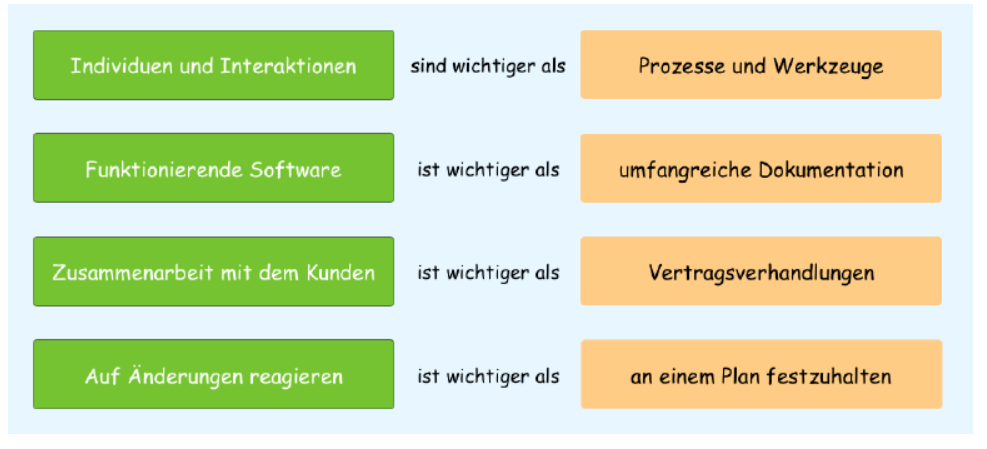
\includegraphics[width=1\textwidth]{figures/daniel/Bild-1.png}
  \caption[]{Scrum Prinzipien verglichen}
  \label{fig:scrum_prinzipien}
\end{figure}

Frei interpretiert wird beim Scrum Framework mehr Wert auf die einzelnen Stakeholder des Projekts gelegt als auf das Projekt selbst. Ebenso werden Bürokratie und Umfangreiche Planungen auf ein nötigstes reduziert. Der Ansatz verfolgt dem klaren Ziel, Teilerfolge schnell sichtbar zu machen und den Kunden in frühen Stadien der Arbeit mit in den Projektfortschritt zu integrieren. 

\subsection{Scrum Rollen}
\subsubsection{Product Owner}
Als Product Owner, am ehesten zum klassischen Projektmanagement mit dem Projektleiter vergleichbar, repräsentiert die Bedürfnisse des Endkunden und steht im engen Austausch mit dem Auftraggeber. Seine Aufgabe ist es, die Bedürfnisse des Kunden genau zu verstehen und diese bestmöglich umsetzen zu lassen. Er hat eine klare Vision und vergleicht Sprintweise den Fortschritt seines Teams und dem resultierenden Inkrement mit der tatsächlichen Wunschsoftware des Kunden. 

\subsubsection{Scrum Master}
Der Scrum Master, ist in dieser Rolle und Funktion einzigartig im gleichnamigen Framework. Er steht für Teamchemie und Prozessreife, gleichzeitig unterstützt er das Team und den Product Owner und gilt als Problemlöser. Der Zauber in seiner Funktion ist die Eigenständigkeit gegenüber dem eigentlichen Product Owner. Er steht als Mittelsmann in vielerlei Hinsicht. Das Team zu verstehen und die Zusammenarbeit und Kommunikation zu verbessern und fördern ist sein Ziel, nicht der direkte Projekterfolg und die Erfüllung der Kundenbedürfnisse.

\subsubsection{Team}
Das Team ist verglichen mit dem klassischen Projektmanagement eher selbstorganisierter und eigenverantwortlicher in der Erfüllung der vom Projektleiter vorgegebenen Aufgaben. Es wird in regelmäßigen Terminen, später näher erläutert viel über Kommunikation und Austausch koordiniert als stets das stumpfe Erledigen von Aufgaben. Das Einbringen von Ideen und das Kundtun von Problemen und Missständen ist essenziell für den Projekterfolg. 


\subsection{Scrum Artefakte}
\subsubsection{Product Backlog}
Das Product Backlog ist am ehesten mit einem Milestoneplan aus dem klassischen Projektmanagement zu vergleichen. Es stellt eine Liste aller offenen Aufgaben dar und wird vom Product Owner gehegt und gepflegt. Er priorisiert hier Sprintweise die zu erledigenden Tätigkeiten nach Wichtigkeit und Dringlichkeit und will für den Kunden den maximal möglichen Umfang rausholen gleichzeitig aber mit enger Abstimmung seines Teams nach deren Möglichkeiten und mit deren technischer Expertise.

\subsubsection{Sprint Backlog}
Der Sprint Backlog ist ein Extrakt aus dem zuvor beschriebenen Product Backlog, reduziert auf die Tätigkeiten eines Sprints. Mit einer Laufzeit von beispielsweise 6 Wochen wird ein gemeinsames Ziel definiert und die dafür zu erfüllenden Aufgaben werden durch den Sprint Backlog als Liste festgehalten. Es erfolgt hier ebenso eine Priorisierung und Zuordnung auf Personen. Die einzelnen Teammitglieder nehmen sich den darin stehenden Aufgaben an und berichtet regelmäßig und eigenständig über den Status der Fertigstellung oder über auftretende Probleme oder benötigte Unterstützung jeglicher Art.

\subsubsection{Product Inkrement}
Das Product Inkrement stellt ein einzelnes Teilergebnis nach einem Sprint dar, auf welches im selbigen hingearbeitet wird. Es soll ein vorzeigbarer und erlebbarer Bestandteil des Gesamtergebnisses sein, welches mit dem Kunden gemeinsam diskutiert wird. Am Produkt Inkrement bekommt das gesamte Team relativ früh und konkret Kundenfeedback über die Zufriedenheit der bisher geleisteten Arbeit. Missverständnisse und Fehler in der Umsetzung sollen sehr schnell aufgezeigt werden.

\subsection{Scrum Events}
\begin{figure}[!htb]
  \centering
  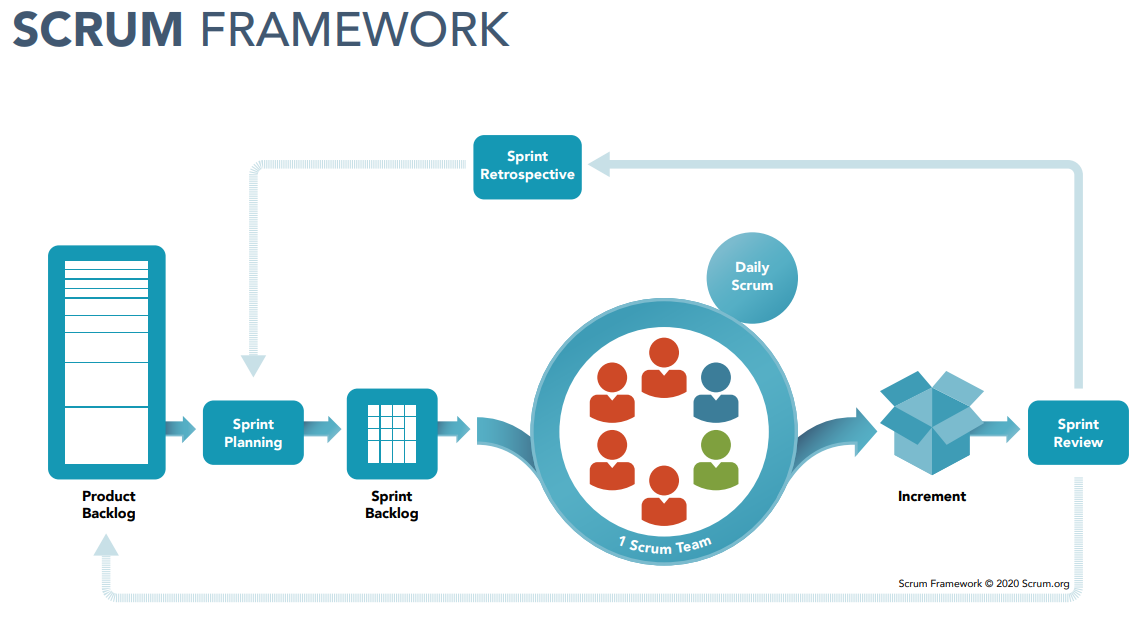
\includegraphics[width=1\textwidth]{figures/daniel/Bild-2.png}
  \caption[]{Scurm-Events im Überblick}
  \label{fig:scrum_events}
\end{figure}

\subsubsection{Sprint}
Der bereits erwähnte Sprint stellt einen Teilabschnitt des Projekts dar. Er besitzt einen eigenen Backlog und wird in der Regel auf 4-8 Wochen terminiert. Innerhalb des Sprints bestimmen weitere Events den Rahmen des Frameworks. Der Sprint selbst steht repräsentativ für das agile Projektmanagement und unterscheidet dich somit klar vom klassischen, oft im Wasserfall ausgelebten Projektmanagement, welches oft nur als Ganzes gesehen wird mit festen Milestones als Einzeletappen.

\subsubsection{Sprint Planning}
Das Sprint Planning stellt den Beginn eines neuen Sprints dar. Hier wird ein Product Inkrement festgelegt, ein gemeinsames Ziel formuliert und deren dafür benötigten Aufgaben definiert. Das Team als Ganzes ist in der Planung involviert. Die Planung selbst erfolgt oftmals über das sogenannte Planning Poker, jedoch kann dieses auch anders praktiziert werden. Jedes einzelne Teammitglied sollte im Austausch mit dem Team selbst und dem Produktowner sowie Scrum Master seinen Arbeitsumfang im Sprint festlegen.



\subsubsection{Weekly Standup}
Das Weekly Standup oftmals auch als Daily Standup praktizierte Event, stellt einen Regeltermin für das gesamte Team dar, in welchem die einzelnen Teammitglieder Ihren aktuellen Arbeitsfortschritt kundtun beziehungsweise kommende Aufgaben und Herausforderungen mit dem Team teilen. Es sollte als kurzes und agiles Event praktiziert werden in welchem auf Probleme und Schwierigkeiten offen und ehrlich mitgeteilt werden. Bei physisch gehaltenen Termin werden die Mitglieder des Termins oft stehend in den Austausch gebracht, online kann dieses zumindest jeder selbst frei entscheiden.

\subsubsection{Sprint Review}
Im Review wird der nun abgeschlossene Sprint begutachtet und der Fortschritt und der Erfolg und Misserfolg objektiv beurteilt. Jedes Mitglied kann seine Aufgaben und Ergebnisse individuell oder als Teil-Team vorstellen und diese gegenüber dem Kunden beziehungsweise dem restlichen Team präsentieren. Es ist darauf zu achten das Event selbst klar von der kommenden Retroperspektive abzugrenzen und persönliche Themen für dieses Event aufzuheben. Der Kunde selbst ist in diesem Event oft involviert.


\subsubsection{Sprint Retrospective}
Die Sprint Retrospective oder auch als Retro bezeichneter Termin, findet gegen Ende des vorangegangenen Sprints statt. Im Gegensatz zum zuvor erwähnten Review werden hier subjektive und zwischenmenschliche Themen miteinander diskutiert. Das Event soll die Möglichkeit schaffen, sich als Team auszutauschen und Gegenseitig mit Lob und konstruktiver Kritik zu konfrontieren. Hier ist vor allem der Scrum Master gefragt ob eine Atmosphäre zu schaffen und das Team zu ermutigen oft auch unangenehme Themen anzusprechen.

\section{Projektmanagement}
\label{sec:projectmanagement}
% \section{Projectmanagement}

In diesem Abschnitt wird der Bereich des Projektmanagements und der Projektplanung innerhalb des Digital Home Town Teams näher erläutert. Als Hilfsmittel wurde hierfür hauptsächlich die Software JIRA von Atlassian verwendet. Hierbei wird auch auf die einzelnen Tasktypen und deren Bedeutung eingegangen. Des Weiteren wurde ein eigener Arbeitsablauf für das Entwicklerteam definiert. Abschließend wird auf die Sprint-Planung und die spätere Verwendung einer sog. User Story Map eingegangen.

\subsection{JIRA}
JIRA ist ein Tool zur Unterstützung von Projektmanagement-Prozessen, das von vielen Unternehmen und Organisationen genutzt wird. Mit JIRA können Projekte geplant, verwaltet und kontrolliert werden, indem Aufgaben, Meilensteine und Prozesse visualisiert und koordiniert werden. Es bietet auch Funktionen zur Zusammenarbeit und Kommunikation innerhalb des Projektteams sowie zur Nachverfolgung von Fortschritten und Problemen. JIRA kann auch individuell angepasst werden, um den spezifischen Bedürfnissen eines Projekts gerecht zu werden. Im Zuge des Projekts wurden mehrere solcher Anpassungen vorgenommen sowie Teaminterne Regeln festgelegt. Diese sollen im Folgenden Abschnitt näher erläutert werden.

\subsubsection{Tasks}
Die Besonderheit an JIRA ist die Möglichkeit zur Aufteilung von mehreren Arbeiten in sogenannte Tasks. Ein Task hat normalerweise eine eindeutige Identifikationsnummer, eine kurze Beschreibung der Aufgabe, eine Zuweisung an einen Verantwortlichen, einen Status sowie ggf. zusätzliche Informationen wie z.B. Verknüpfungen mit anderen Tasks. 

\begin{figure}[ht!]
    \centering
    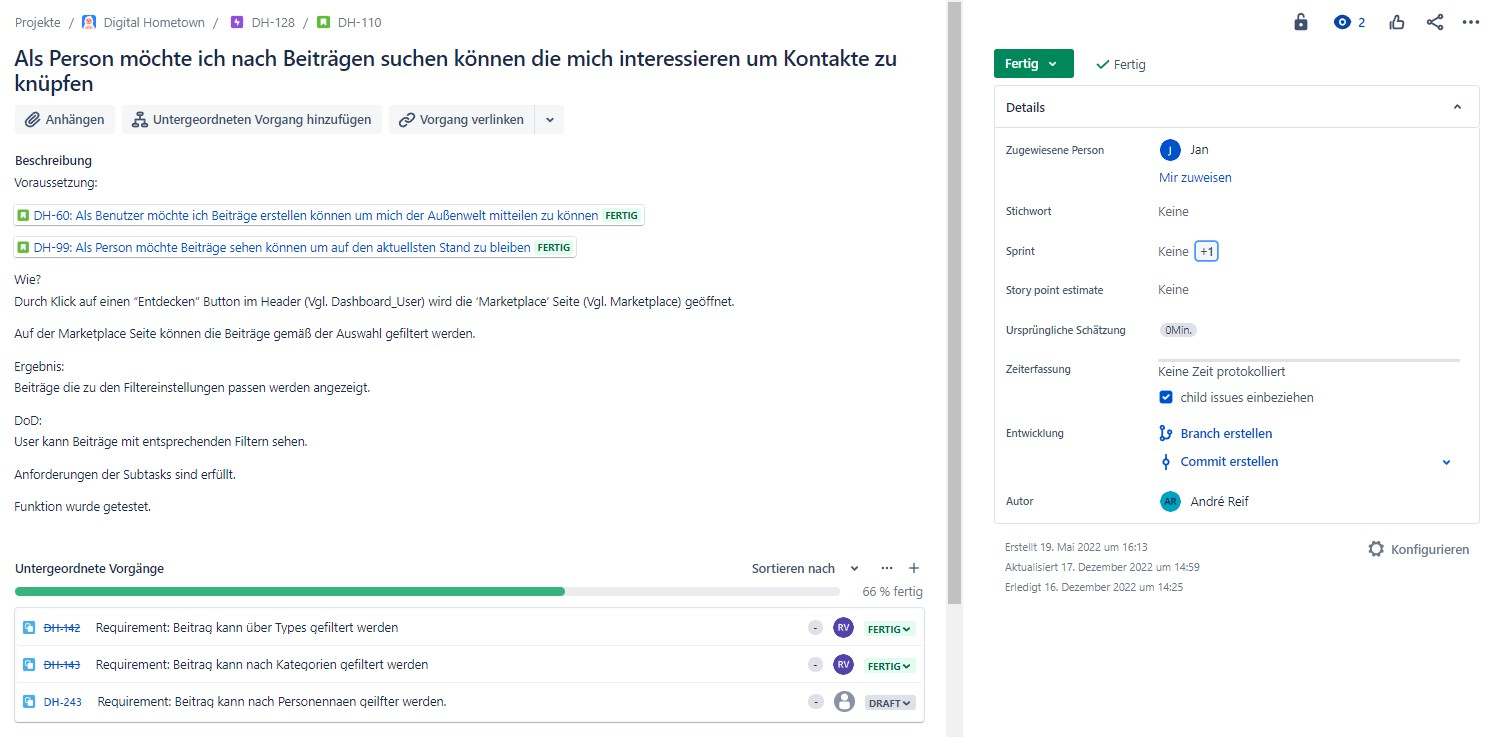
\includegraphics[width=0.6\textwidth]{figures/andre/jiratask.jpg}
    \caption{Beispiel für einen Task im JIRA}
    \label{fig:jiratask}
\end{figure}

Einzelne Tasks können in sog. Epics geclustert werden, um so die Aufgaben und langfristige Planung besser strukturieren zu können. Im Folgenden ist eine Übersicht der Epics innerhalb des Projekts sowie deren Fortschritt zu sehen.

\begin{figure}[ht!]
    \centering
    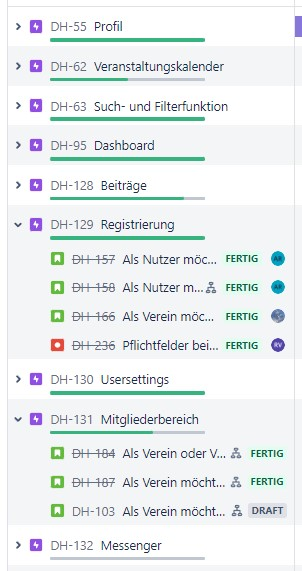
\includegraphics[width=0.6\textwidth]{figures/andre/epicsdesprojekts.jpg}
    \caption{Epic Übersicht des Projekts}
    \label{fig:epicsdesprojekts}
\end{figure}

Für die einzelnen Tasks wurden jeweils 4 verschiedene Typen unterschieden.

\subsubsection*{User-Story}
Eine User Story beschreibt eine neue Nutzeranforderung, also ein Feature, dass umgesetzt werden muss das der Benutzer die entsprechende Tätigkeit ausführen kann. Diese werden per Definition nach dem folgenden Prinzip geschrieben:

Als Nutzer möchte ich \textbf{<Auszuführende Tätigkeit>} um \textbf{<Vorteil oder Intention der ausgeführten Tätigkeit>}.

Eine User Story hat den Folgenden Aufbau:
\begin{itemize}
    \item \textbf{Titel} User Story nach Definition.
    \item \textbf{Wie?} Kurze Beschreibung wie die Funktion umgesetzt werden soll.
    \item \textbf{Ergebnis?} Beschreibung was passiert, wenn die Funktion ausgeführt wird.
    \item \textbf{DoD} Definition of Done, also eine Definition, wann der Task als erledigt gilt.
\end{itemize}

\subsubsection*{Sub-Task}
Sub-Tasks werden in der Regel dazu verwendet, um besonders aufwendige User Stories und Tasks in kleinere Arbeitseinheiten zu unterteilen. Für Digital Home Town wurden die Sub-Tasks verwendet, um Task-spezifische Anforderungen zu dokumentieren und hervorzuheben. 
\subsubsection*{Functional-Task}
Für unterstützende Arbeiten, die nicht direkt mit der Entwicklung der Plattform in Verbindung stehen, wurden sog. Functional Tasks eingeführt. Diese sind in der Regel nicht näher definiert oder Beschrieben und sind Anhand des Titels nachvollziehbar. 

\begin{figure}[ht!]
    \centering
    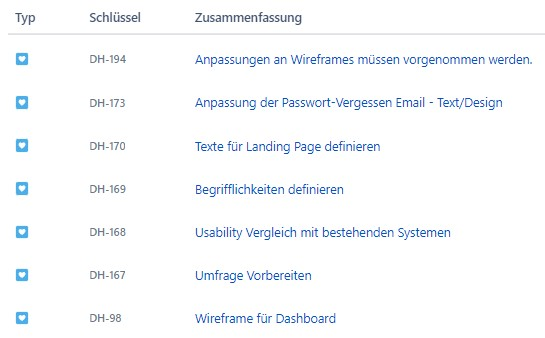
\includegraphics[width=0.6\textwidth]{figures/andre/functionaltasks.jpg}
    \caption{Beispiele für Functional Tasks}
    \label{fig:functionaltasks}
\end{figure}

\subsubsection*{Bug}
Ein Bug stellt einen gefundenen Fehler auf der Plattform da. Dieser spiegelt sowohl einen Fehlerbericht als auch einen neuen Arbeitsauftrag dar. Innerhalb des Entwicklerteams war es üblich, dass zumeist der Verursacher des Bugs auch für dessen Behebung verantwortlich war. Ein Bug durchläuft allerdings denselben Arbeitsablauf wie eine User-Story und nach den gleichen Standards getestet.

\begin{figure}[ht!]
    \centering
    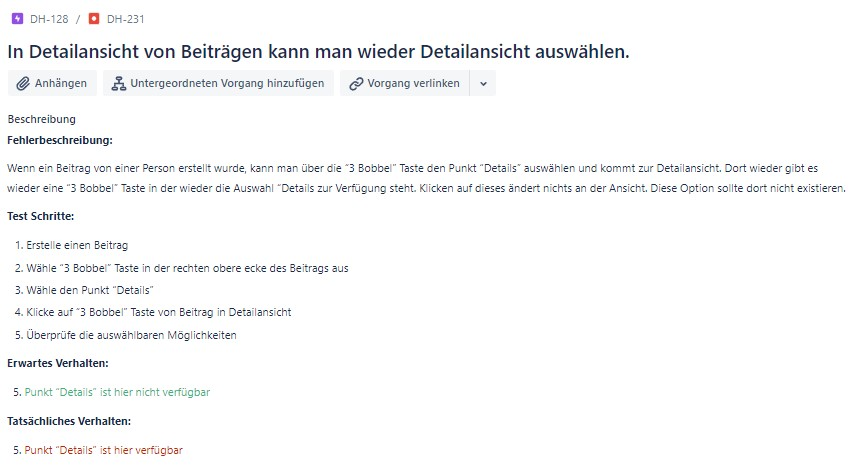
\includegraphics[width=0.6\textwidth]{figures/andre/bugticket.jpg}
    \caption{Beispiel für ein Bug Ticket}
    \label{fig:bugticket}
\end{figure}

Ein Bug besteht in der Regel aus:

\begin{itemize}
    \item \textbf{Titel} Kurze Beschreibung des Fehlers
    \item \textbf{Beschreibung} Detaillierte Beschreibung des Fehlers und des Fehlerhergangs
    \item \textbf{Test Schritte} Schritt-für-Schritt Angaben über den Ablauf des Tests
    \item \textbf{Verhalten} Erwartetes und Tatsächliches Verhalten
\end{itemize}

\subsubsection{Arbeitsablauf}
In der folgenden Abbildung ist der Allgemeine Arbeitsablauf für ein einzelnes JIRA Ticket zu sehen.

\begin{figure}[h!]
    \centering
    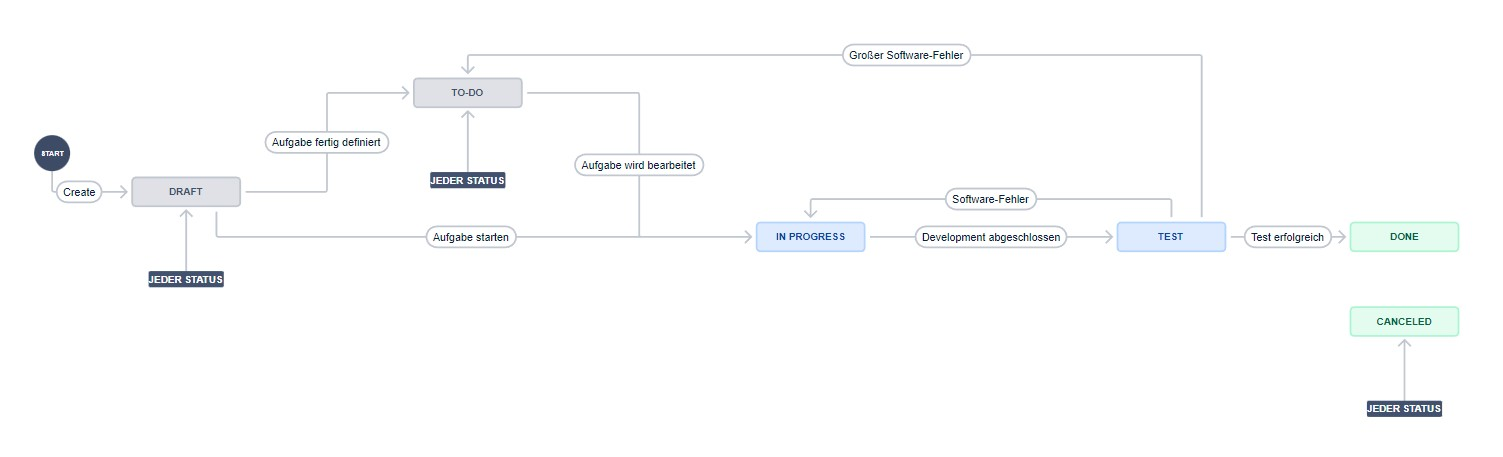
\includegraphics[width=0.6\textwidth]{figures/andre/workflow.jpg}
    \caption{Darstellung des Ablaufs eines einzelnen JIRA Tickets}
    \label{fig:workflow}
\end{figure}

Ein einzelner Task wurde zunächst mit dem Status „Draft“ erstellt. Dies wurde im Allgemeinen so interpretiert, dass das Ticket zwar angelegt wurde, jedoch nicht vom Team so akzeptiert wurde, dass jeder die Aufgabe verstanden hat. Dies wurde bei der Sprint Planung bzw. dem Task Refinement während der Planung Besprochen, ggf. angepasst, und dann festgelegt. 

Nachdem ein Task den Status „ToDo“ erhält, kann dieser in einem Sprint eingeplant und entsprechend bearbeitet werden. Der Status wechselt demnach zu „In Progress“. 

Nach der Bearbeitung wird ein Ticket mit Hilfe des Flags „Test“ zum Testen freigegeben. Das Bedeutet der Code läuft in der Entwicklungsumgebung und kann von einem Tester bearbeitet werden. Ob im Fehlerfall ein Task zurück in den Status „ToDo“ oder „In Progress“ versetzt wurde, lag in der Schwere des Fehlers und im Ermessen des jeweiligen Testers. Falls der Test erfolgreich war, wurde der Task auf den Status „Done“ verschoben und war somit abgearbeitet.

Aufgrund sich ändernder Anforderungen wurde später der „Canceled“ Staus eingeführt, um ggf. bereits begonnene Tasks abbrechen zu können.

Dieser Ablauf gilt in der Regel für jede User Story sowie jeden Bug. Die Stati „Draft“ und „Test“ hatten für Functional Tasks und Sub Tasks jedoch keine tiefergehende Bedeutung und konnten einfach übersprungen werden.

\subsection{Sprint Planning mit JIRA}
Die Sprints wurden in der Regel vorausgeplant. Dabei galt die Regel: der nächste Sprint steht am Ende des aktuellsten Sprints weitestgehend fest, der übernächste Sprint ist zu 50\% geplant. 

Während der Planungsmeetings wurden die geplanten Tasks und Bugs besprochen und auf deren Umsetzbarkeit und Priorität geprüft. Aufgrund der un-terschiedlichen Kenntnisse und Fertigkeiten der Entwickler war es jedoch schwierig den Aufwand einzelner Tasks verallgemeinert für das gesamte Entwicklungsteam einzuschätzen. Zuzüglich dazu mussten Urlaubs- und Abwesenheitszeiten bei der Planung berücksichtigt werden, sodass die definierten Sprint Ziele auch erreicht werden konnten.

\begin{figure}[h!]
    \centering
    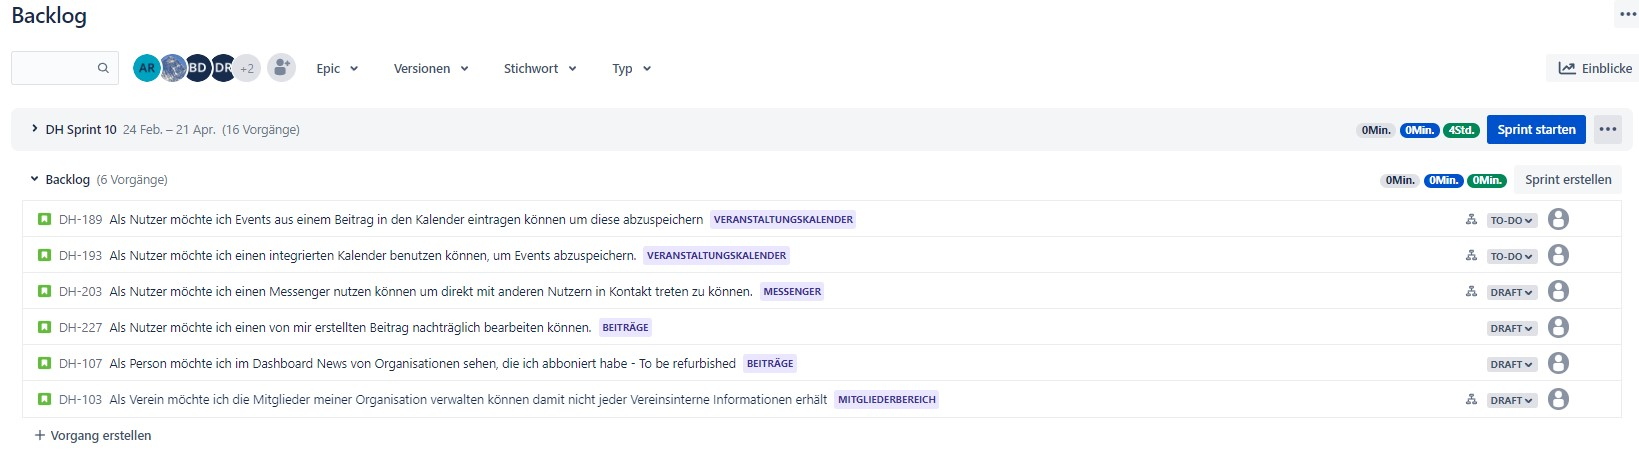
\includegraphics[width=0.6\textwidth]{figures/andre/jirabacklog.jpg}
    \caption{Backlog Funktion im JIRA}
    \label{fig:jirabacklog}
\end{figure}

Zur Planung der Sprints wurde die in der obigen Abbildung zu sehende Backlog Funktion verwendet. Hier sind zum sowohl die nicht geplanten Tasks zu sehen als auch die einem Sprint bereits zugeordnetem Task und können auch bei Bedarf entsprechend umgeplant werden. So war es nicht unüblich, dass nachdem das Sprintziel bereits vor dem Ende des Sprints erreicht wurde, noch offene Bugs oder kleinere Functional Tasks dem Sprint hinzugefügt und abgearbeitet wurden. Zum Sprintende begonnene Arbeitsaufträge wurden grundsätzlich in den nachfolgenden Sprint verschoben und fertiggestellt.

\subsubsection{User Story Map}
Als weiteres Tool zur Projektplanung wurde der Ansatz des sogenannten User Story Mapping verwendet. Per Definition ist eine User Story Map eine Technik zur Visualisierung von Benutzeranforderungen und -funktionen in einer hierarchischen Struktur.

\begin{figure}[h!]
    \centering
    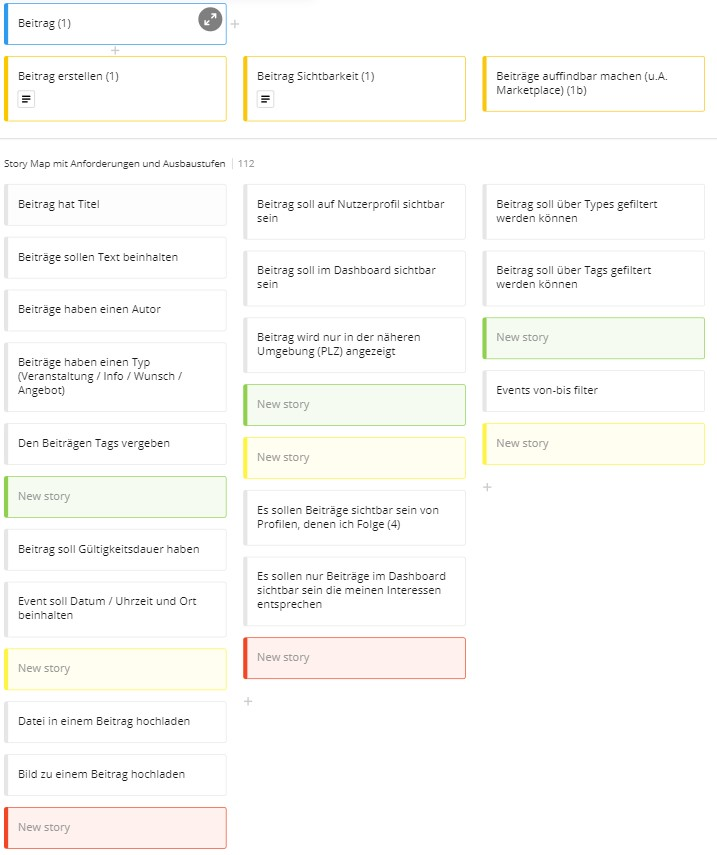
\includegraphics[width=0.6\textwidth]{figures/andre/userstorymap.jpg}
    \caption{Beiträge in der User Story Map}
    \label{fig:userstorymap}
\end{figure}

In der obigen Abbildung ist die User Story Map für einige Features der Beiträge zu finden. So gibt es zur User Story „Als Nutzer möchte ich einen Beitrag erstellen können um mich der Community mitteilen zu können“ verschiedene Anforderungen. Diese stehen unterhalb des jeweils gelben Blocks. 

Die Anforderungen jeweils wurden dann in 3 Iterationsstufen Priorisiert:

\begin{itemize}
    \item \textbf{Bis Grün} Minimum viable product, also die Minimalanforderungen die Umgesetzt werden sollen
    \item \textbf{Bis Gelb} Nice-to-Have, Anforderungen die umgesetzt werden sollen, aber nicht hoch Priorisiert werden
    \item \textbf{Bis Rot} Wird implementiert falls genügend Zeit dafür da ist
\end{itemize}

Aus dieser Map wurden dann die einzelnen User Story Tasks im JIRA angelegt und entsprechend in den Sprints verplant.

\section{Sprintübersicht}
\label{sec:sprintoverview}
\input{content/03_process/03_Sprintübersicht}
